% Datenblatt skAInet Edge-Compute v1.5
\documentclass[10pt,a4paper]{article}
\usepackage[margin=20mm,top=18mm,bottom=20mm]{geometry}
\usepackage[T1]{fontenc}
\usepackage[utf8]{inputenc}
\usepackage[ngerman]{babel}
\usepackage{helvet}\renewcommand{\familydefault}{\sfdefault}
\usepackage{booktabs,array,tabularx,siunitx,microtype}
\usepackage{tikz}
\usetikzlibrary{calc,arrows.meta}
\usepackage{xcolor}
\usepackage{graphicx}
\definecolor{skred}{HTML}{C8102E}
\definecolor{skgray}{HTML}{444444}
\usepackage{fancyhdr}
\pagestyle{fancy}\fancyhf{}
\fancyhead[L]{\small\textbf{skAInet Edge-Compute v1.5} — Datenblatt}
\fancyhead[R]{\small Auto-Intern GmbH, Bochum}
\fancyfoot[L]{\small DB-EC-1.5 · September 2026}
\fancyfoot[R]{\small Seite \thepage}
\renewcommand{\headrulewidth}{0.4pt}
\setlength{\parindent}{0pt}
\sisetup{locale=DE, per-mode=symbol}

% Bemaßungs-Makros
\tikzset{
  dimline/.style={<->, >=Latex, line width=0.4pt, draw=skgray},
  extline/.style={line width=0.3pt, draw=skgray},
  dimtext/.style={fill=white, inner sep=1pt, font=\footnotesize, text=black},
  part/.style={line width=0.8pt, draw=black},
  hidden/.style={line width=0.4pt, draw=skgray, dash pattern=on 2pt off 1.5pt},
  center/.style={line width=0.3pt, draw=skgray, dash pattern=on 6pt off 1.5pt on 1pt off 1.5pt},
}

\begin{document}

%=====================================================================
% Seite 1 — Übersicht & Spezifikation
%=====================================================================
\begin{minipage}[b]{0.66\textwidth}
{\LARGE\textbf{\textcolor{skred}{skAInet} Edge-Compute}}\quad{\Large v1.5}

\vspace{2mm}
{\large Programmierbarer M12-PoE-Switch, Router und Linux-Compute-Modul für die industrielle Edge-Datenerfassung}
\end{minipage}\hfill
\begin{minipage}[b]{0.26\textwidth}
\raggedleft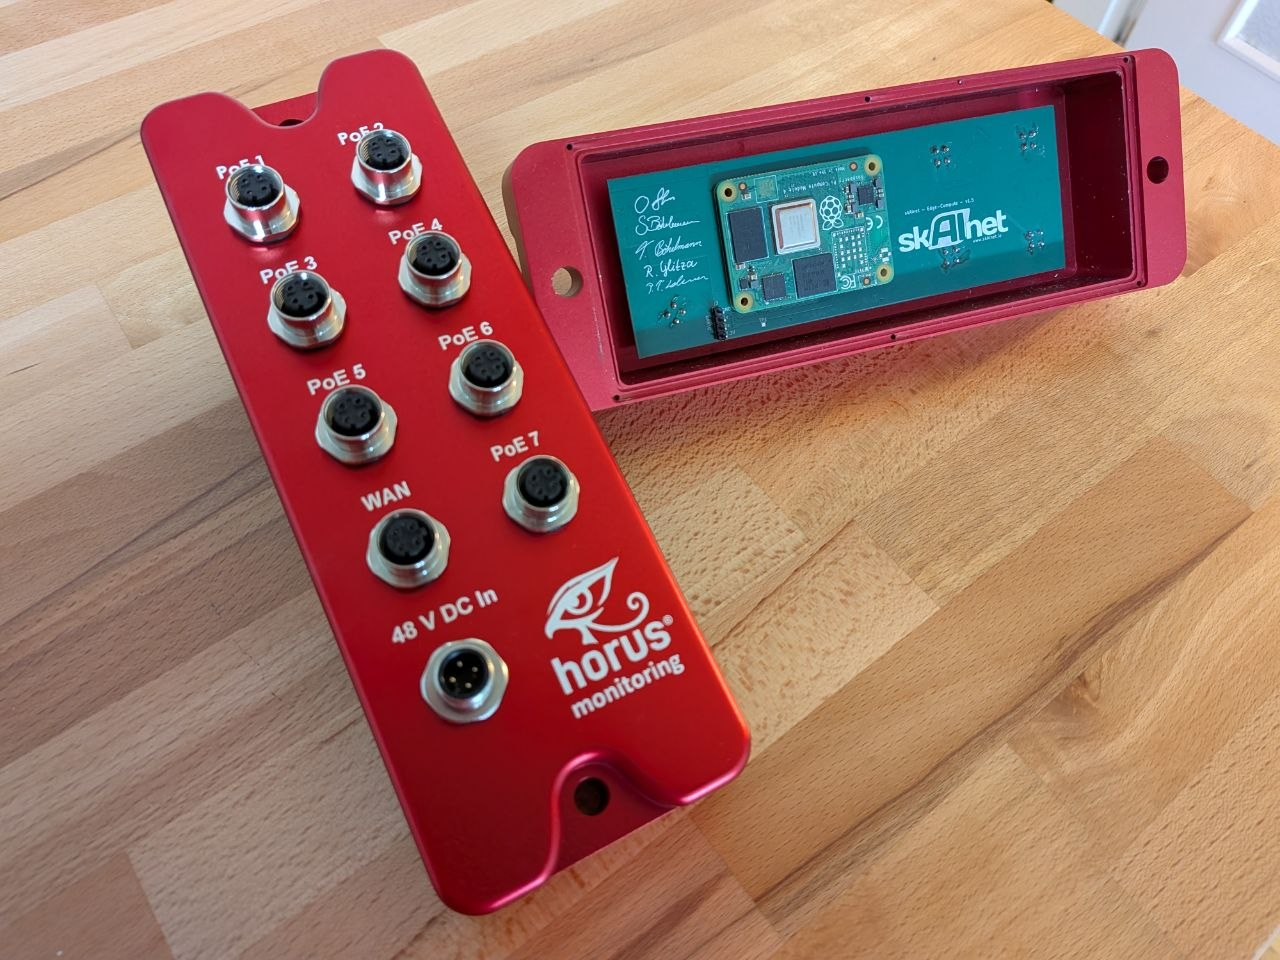
\includegraphics[width=\textwidth]{edge-branded.jpg}
\end{minipage}

\vspace{2mm}\hrule\vspace{2mm}

\textbf{Kurzbeschreibung.} Der skAInet Edge-Compute ist die universelle
Datenerfassungs- und Monitoring-Plattform der Auto-Intern GmbH. Ein
eloxiertes Aluminiumgehäuse, aus einem Block gefräst, vereint einen
8-Port-Switch mit sieben nach außen geführten M12-PoE+-LAN-Ports
(D-codiert), einen separaten M12-WAN-Port (D-codiert) und ein
wechselbares Compute-Modul (Raspberry-Pi-CM-pinkompatibel). Alle
Anschlüsse sind als dichtende M12-Steckverbinder ausgeführt; das Gerät
ist bis \SI{1}{bar} unter Wasser betreibbar. Messdaten werden auf dem
Gerät gepuffert, vorverarbeitet und analysiert; in das übergeordnete
Netz gelangen nur die Daten, deren Weiterleitung konfiguriert wurde.

\vspace{2mm}
\begin{minipage}[t]{0.48\textwidth}
\textbf{Compute}\par\vspace{1mm}
\begin{tabularx}{\textwidth}{@{}>{\bfseries}p{2.9cm}X@{}}
\toprule
Modul & Raspberry Pi CM4 (Standard); CM5 oder NVIDIA Jetson auf Anfrage, pinkompatibel wechselbar \\
CPU & 8\,Kerne, 64-bit ARM, \SI{1.5}{GHz} \\
RAM & \SI{8}{GB} LPDDR4-3200 \\
Speicher & \SI{32}{GB} eMMC \\
Betriebssystem & Yocto Linux, dokumentierte SBOM (EU Cyber Resilience Act); verschlüsselte OTA-Updates oder offline per USB-Image \\
\bottomrule
\end{tabularx}

\vspace{2mm}
\textbf{Netzwerk}\par\vspace{1mm}
\begin{tabularx}{\textwidth}{@{}>{\bfseries}p{2.9cm}X@{}}
\toprule
WAN & 1$\times$ M12 D-codiert (4-polig), Gigabit-Ethernet, DHCP-Client \\
LAN & 7$\times$ M12 D-codiert (4-polig, Ethernet) mit PoE+, intern an 8-Port-Switch (DHCP-Server, 192.168.199.1/24) \\
PoE & IEEE~802.3at (PoE+) auf allen 7 LAN-Ports; typ. Geräte bis ca. \SI{10}{W} \\
Verkabelung & 1 zertifiziertes Cat-5e-M12-Kabel je Gerät \\
Datenschnittstelle & Live-Daten via WebSocket (Port 8001, JSON, ns-Zeitstempel) \\
Upstream-APIs & REST, WebSocket, Webhooks, MQTT, OPC~UA, Modbus-TCP, EPICS, gRPC, AMQP, CoAP, SNMP, Prometheus, InfluxDB, SFTP/rsync \\
Kapazität & 250+ parallele Kanäle im Produktivbetrieb nachgewiesen \\
\bottomrule
\end{tabularx}
\end{minipage}\hfill
\begin{minipage}[t]{0.48\textwidth}
\textbf{Versorgung}\par\vspace{1mm}
\begin{tabularx}{\textwidth}{@{}>{\bfseries}p{2.9cm}X@{}}
\toprule
Eingang & \SIrange{48}{72}{V} DC über M12 A-codiert (4-polig, TE T4140012041-000) \\
Netzteil & empfohlen $\geq$ \SI{100}{W} \\
Minimal & \SI{25}{W} (nur Compute, ohne PoE-Lasten) \\
\bottomrule
\end{tabularx}

\vspace{2mm}
\textbf{Umgebung \& Mechanik}\par\vspace{1mm}
\begin{tabularx}{\textwidth}{@{}>{\bfseries}p{2.9cm}X@{}}
\toprule
Gehäuse & eloxiertes Aluminium, aus dem Vollen, stoßfest \\
Schutzart & IP67, alle Ports und Rückplatte gedichtet; Betrieb bis \SI{1}{bar} unter Wasser \\
Temperatur & \SIrange{-25}{70}{\celsius} \\
Abmessungen & $216 \times 75 \times 32$ \si{mm} (B$\times$T$\times$H); Gesamttiefe inkl.\ Steckverbinder ca.\ \SI{51}{mm} \\
Frontplatte & 8$\times$ M12 D-codiert (7$\times$ PoE-LAN, 1$\times$ WAN) im 4$\times$2-Raster, 1$\times$ M12 A-codiert Power-In; kundenspezifisches Branding möglich \\
\bottomrule
\end{tabularx}

\vspace{2mm}
\textbf{Software}\par\vspace{1mm}
\begin{tabularx}{\textwidth}{@{}>{\bfseries}p{2.9cm}X@{}}
\toprule
Zugriff & SSH (Port 22022); eigene Anwendungen in C++ oder Python, Docker-Deployment; Minimalbeispiele auf GitHub \\
Fernwartung & optionale, abschaltbare Hersteller-Fernwartung über verschlüsselten Zugang \\
Updates & verschlüsselte OTA-Updates über den WAN-Port oder offline per USB-Image \\
\bottomrule
\end{tabularx}

\vspace{2mm}
\textbf{Referenz-Einsätze}\par\vspace{1mm}
{\small DB Netz DIANA (Weichenmotor-Monitoring) · Kelvion (IR-Fouling-Erkennung) · Kurtz Ersa / Global Point HORUS (Lötprozess-Monitoring) · RUB/GSI-FAIR PANDA (Luminositätsdetektor) · MSU CBE (Fluss-Impedanzspektroskopie) · NexuFed AI / RUB (föderiertes Pumpen-Monitoring)}
\end{minipage}

\vspace{2mm}\hrule\vspace{1.5mm}
{\small
\textbf{Hersteller:} Auto-Intern GmbH · Herner Str.\ 299, Gebäude B29, 44809 Bochum · info@auto-intern.de · +49\,234\,9345\,1121\\
\textbf{Preis:} ab 260\,€ / 299\,\$ netto · \textbf{Dokumentation:} edge-compute.skainet.io}

%=====================================================================
% Seite 2 — Bemaßte Zeichnung (vollseitig)
%=====================================================================
\newpage
\thispagestyle{fancy}
%=====================================================================
% Seiten 2-4 — Maßzeichnung 1:1, je Ansicht eine Seite, Modul vertikal
%=====================================================================
\begin{center}
{\large\textbf{Maßzeichnung — Gehäuse Edge-Compute v1.5}}\\[1mm]
{\small Alle Maße in mm · Allgemeintoleranz ISO 2768-mK · Werkstoff: Al, eloxiert · \textbf{Maßstab 1:1} · Blatt 1/4: Frontansicht}
\end{center}
\vfill
\begin{center}
\begin{tikzpicture}[scale=0.1, rotate=90]  % 1:1, Modul vertikal
  % Außenkontur 216 x 75, Eckradius 10
  \draw[part, rounded corners=1cm] (-108,-37.5) rectangle (108,37.5);
  \draw[center] (-114,0) -- (114,0);
  \draw[center] (0,-43) -- (0,43);
  % M12-Buchsen D-codiert: Kontur Ø16 mit Abflachungen, Raster 4x2, Teilung 32/32
  \foreach \x in {-64,-32,0,32}{
    \foreach \y in {-16,16}{
      \begin{scope}[shift={(\x,\y)}]
        \draw[part] (6.75,{sqrt(64-6.75*6.75)}) arc[start angle={acos(6.75/8)}, end angle={180-acos(6.75/8)}, radius=8];
        \draw[part] (-6.75,{-sqrt(64-6.75*6.75)}) arc[start angle={180+acos(6.75/8)}, end angle={360-acos(6.75/8)}, radius=8];
        \draw[part] (6.75,{sqrt(64-6.75*6.75)}) -- (6.75,{-sqrt(64-6.75*6.75)});
        \draw[part] (-6.75,{sqrt(64-6.75*6.75)}) -- (-6.75,{-sqrt(64-6.75*6.75)});
        \draw[part] (0,0) circle[radius=6];
        \draw[part] (0,0) circle[radius=4.5];
        \foreach \a in {45,135,225,315} \fill (\a:2.6) circle[radius=0.6];
        \draw[center] (-10,0)--(10,0); \draw[center] (0,-10)--(0,10);
      \end{scope}
    }
  }
  % Power-Buchse A-codiert, 45° gedreht, Position (80, -16)
  \begin{scope}[shift={(64,-16)}, rotate=45]
    \draw[part] (6.75,{sqrt(64-6.75*6.75)}) arc[start angle={acos(6.75/8)}, end angle={180-acos(6.75/8)}, radius=8];
    \draw[part] (-6.75,{-sqrt(64-6.75*6.75)}) arc[start angle={180+acos(6.75/8)}, end angle={360-acos(6.75/8)}, radius=8];
    \draw[part] (6.75,{sqrt(64-6.75*6.75)}) -- (6.75,{-sqrt(64-6.75*6.75)});
    \draw[part] (-6.75,{sqrt(64-6.75*6.75)}) -- (-6.75,{-sqrt(64-6.75*6.75)});
    \draw[part] (0,0) circle[radius=6];
    \draw[part] (0,0) circle[radius=4.5];
    \foreach \a in {45,135,225,315} \fill (\a:2.6) circle[radius=0.6];
    \draw[center] (-10,0)--(10,0); \draw[center] (0,-10)--(0,10);
  \end{scope}
  \node[font=\scriptsize, text=skgray, anchor=west] at (64,-40) {Power-In (M12 A-cod., 4-pol.), 45°};
  % Bemaßung 216 (nach Rotation vertikal)
  \draw[extline] (-108,37.5) -- (-108,48);
  \draw[extline] (108,37.5) -- (108,48);
  \draw[dimline] (-108,45) -- (108,45) node[dimtext,midway,rotate=90]{216};
  % Bemaßung 75 (nach Rotation horizontal)
  \draw[extline] (-108,-37.5) -- (-119,-37.5);
  \draw[extline] (-108,37.5) -- (-119,37.5);
  \draw[dimline] (-116,-37.5) -- (-116,37.5) node[dimtext,midway]{75};
  % Raster-Teilung 32
  \draw[extline] (-64,-16) -- (-64,-48);
  \draw[extline] (-32,-16) -- (-32,-48);
  \draw[dimline] (-64,-45) -- (-32,-45) node[dimtext,midway,rotate=90]{32};
  \draw[extline] (0,16) -- (0,52);
  \draw[extline] (32,16) -- (32,52);
  \draw[dimline] (0,49) -- (32,49) node[dimtext,midway,rotate=90]{32 (4$\times$)};
  \draw[extline] (-64,16) -- (-86,16);
  \draw[extline] (-64,-16) -- (-86,-16);
  \draw[dimline] (-83,-16) -- (-83,16) node[dimtext,midway]{32};
  % Beschriftungen
  \node[dimtext, anchor=west] at (-95,44) {8$\times$ M12 D-codiert (Ethernet, 4-pol.)};
  \draw[extline] (-88,42) -- (-70,18);
  \node[dimtext] at (100,25) {R10 (4$\times$)};
  % 2x Ø8,5 Montagebohrungen in den Laschen (bei ±98, mittig)
  \foreach \x in {-98,98}{
    \draw[part] (\x,0) circle[radius=4.25];
    \draw[center] (\x-8,0)--(\x+8,0); \draw[center] (\x,-8)--(\x,8);
  }
  \draw[extline] (-98,0) -- (-98,-55);
  \draw[extline] (98,0) -- (98,-55);
  \draw[dimline] (-98,-52) -- (98,-52) node[dimtext,midway,rotate=90]{196};
  \node[dimtext, anchor=east] at (93,-14) {2$\times$ Ø8{,}5 (Montage)};
  \node[font=\small\bfseries, rotate=90] at (0,-62) {Frontansicht — Steckverbinderseite};
\end{tikzpicture}
\end{center}
\vfill

\newpage
\thispagestyle{fancy}
\begin{center}
{\small Alle Maße in mm · \textbf{Maßstab 1:1} · Blatt 2/4: Bodenansicht}
\end{center}
\vfill
\begin{center}
\begin{tikzpicture}[scale=0.1, rotate=90]
  \draw[part, rounded corners=1cm] (-108,-37.5) rectangle (108,37.5);
  \draw[center] (-114,0) -- (114,0);
  \draw[center] (0,-43) -- (0,43);
  % Tasche 166x58 R3 t30
  \draw[hidden, rounded corners=0.3cm] (-83,-29) rectangle (83,29);
  % 6x M3x30 Deckelverschraubung
  \foreach \x in {-70,0,70}{
    \foreach \y in {-25,25}{
      \draw[part] (\x,\y) circle[radius=1.5];
      \draw[center] (\x-4,\y)--(\x+4,\y); \draw[center] (\x,\y-4)--(\x,\y+4);
    }
  }
  % Bemaßung
  \draw[extline] (-83,-29) -- (-83,-50);
  \draw[extline] (83,-29) -- (83,-50);
  \draw[dimline] (-83,-47) -- (83,-47) node[dimtext,midway,rotate=90]{166 (Tasche, t=30, R3)};
  \draw[extline] (-83,29) -- (-119,29);
  \draw[extline] (-83,-29) -- (-119,-29);
  \draw[dimline] (-116,-29) -- (-116,29) node[dimtext,midway]{58};
  \draw[extline] (-108,37.5) -- (-108,48);
  \draw[extline] (108,37.5) -- (108,48);
  \draw[dimline] (-108,45) -- (108,45) node[dimtext,midway,rotate=90]{216};
  \node[dimtext, anchor=west] at (-60,-38) {6$\times$ M3$\times$30 (Deckelverschraubung)};
  \draw[extline] (-55,-36) -- (-68.5,-26.5);
  \node[font=\small\bfseries, rotate=90] at (0,-60) {Bodenansicht — Tasche und Deckelverschraubung};
\end{tikzpicture}
\end{center}
\vfill

\newpage
\thispagestyle{fancy}
\begin{center}
{\small Alle Maße in mm · \textbf{Maßstab 1:1} · Blatt 3/4: Seitenansicht}
\end{center}
\begin{center}
\begin{tikzpicture}[scale=0.1, rotate=90]
  % Profil: Basis 20 + Deckel 12 = 32
  \draw[part] (-108,0) -- (108,0) -- (108,32) -- (-108,32) -- cycle;
  \draw[hidden] (-108,20) -- (108,20);
  % M12-Steckverbinder (Überstand 19: Sechskant, Gewindekörper, Kupplungsring)
  \foreach \x in {-64,-32,0,32,64}{
    \draw[part] (\x-9,32) -- (\x-9,36) -- (\x-7.5,36) -- (\x-7.5,44)
      -- (\x-8,44) -- (\x-8,51) -- (\x+8,51) -- (\x+8,44)
      -- (\x+7.5,44) -- (\x+7.5,36) -- (\x+9,36) -- (\x+9,32);
    \draw[center] (\x,30) -- (\x,54);
  }
  \node[dimtext, rotate=90, anchor=west] at (80,56) {M12 (9$\times$)};
  % Bemaßung Höhen
  \draw[extline] (108,0) -- (117,0);
  \draw[extline] (108,20) -- (117,20);
  \draw[extline] (108,32) -- (117,32);
  \draw[extline] (88,51) -- (117,51);
  \draw[dimline] (114,0) -- (114,20) node[dimtext,midway]{20};
  \draw[dimline] (114,20) -- (114,32) node[dimtext,midway]{12};
  \draw[dimline] (114,32) -- (114,51) node[dimtext,midway]{19};
  \draw[extline] (-108,0) -- (-117,0);
  \draw[extline] (-108,32) -- (-117,32);
  \draw[dimline] (-114,0) -- (-114,32) node[dimtext,midway]{32};
  \draw[extline] (-108,0) -- (-108,-9);
  \draw[extline] (108,0) -- (108,-9);
  \draw[dimline] (-108,-6) -- (108,-6) node[dimtext,midway,rotate=90]{216};
  \node[dimtext, rotate=90] at (30,16) {Deckelprofil mit Griffmulde, Kantenradius R3};
  \node[font=\small\bfseries, rotate=90] at (0,-18) {Seitenansicht};
\end{tikzpicture}
\end{center}

\newpage
\thispagestyle{fancy}
\begin{center}
{\small Blatt 4/4: Isometrie des Compute-Moduls, Steckverbinderseite (nicht maßstäblich)}
\end{center}
\vfill
\begin{center}
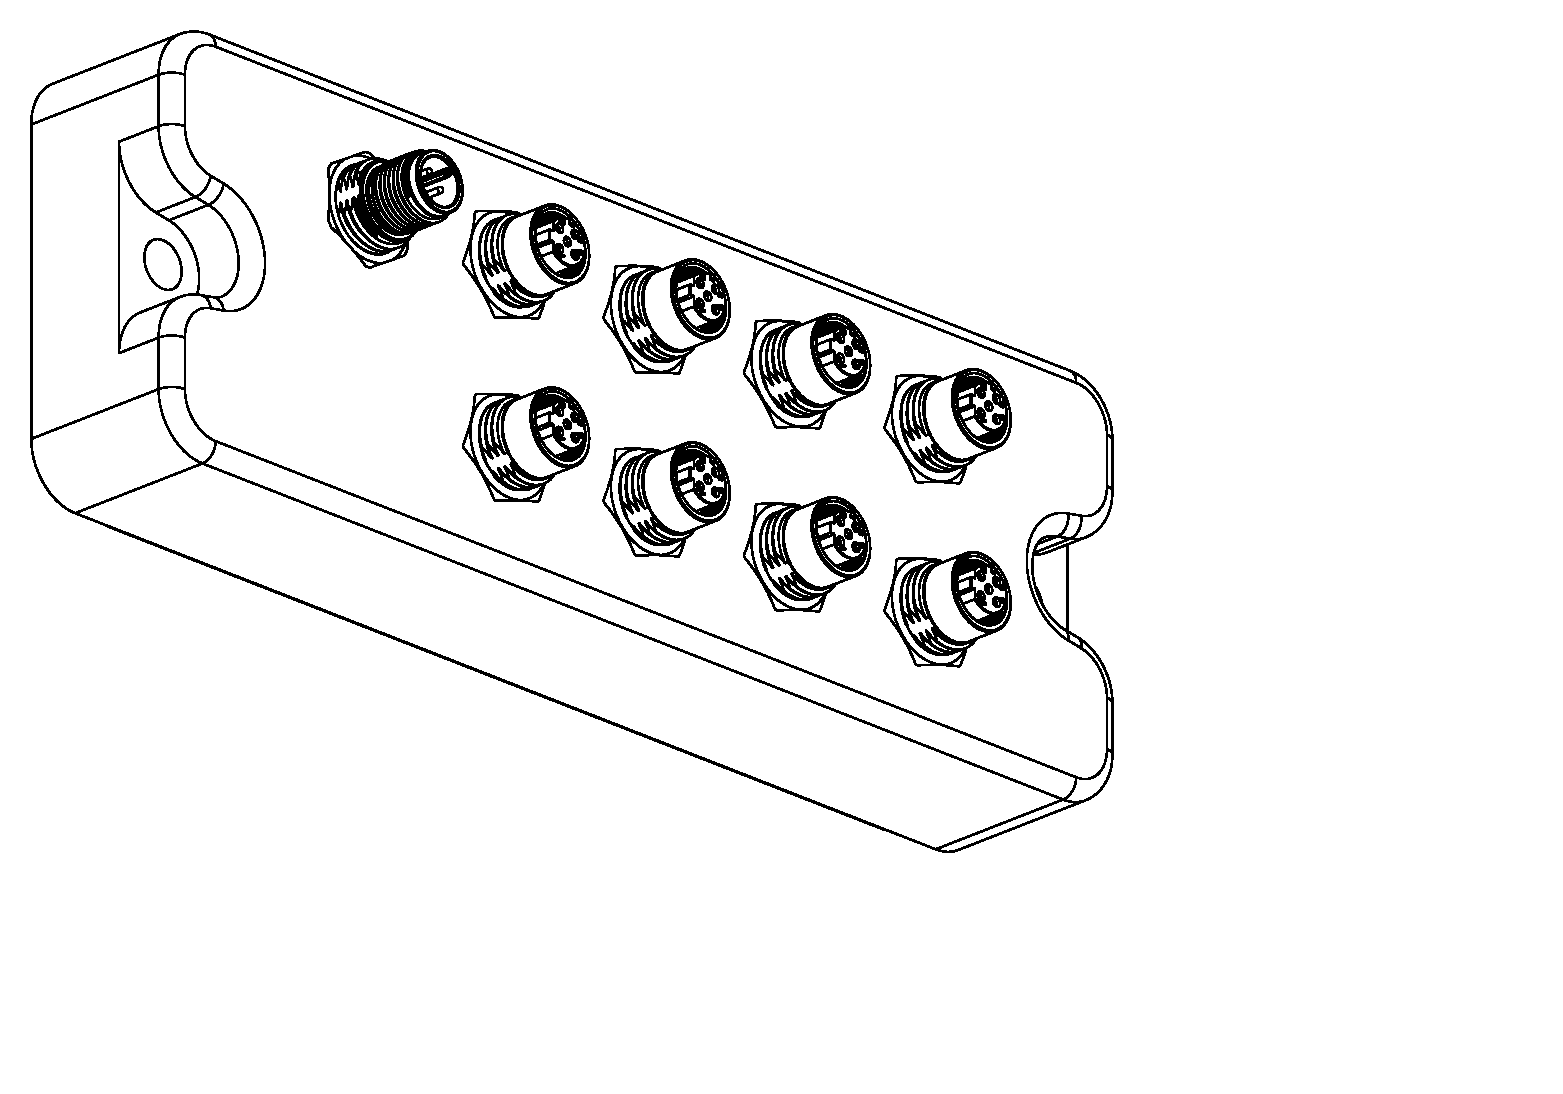
\includegraphics[width=0.95\textwidth]{horus-assembly.pdf}
\end{center}
\vfill
{\scriptsize Alle Steckverbinder M12, IP67: 8$\times$ D-codiert (7$\times$ PoE-LAN, 1$\times$ WAN, 4-polig Ethernet), Teilung $32\times32$; 1$\times$ A-codiert Power-In (4-polig), 45° gedreht. Deckelbefestigung: 6$\times$ M3$\times$30. Angaben ohne Gewähr.}

\end{document}
